\subsection{度量空间的结构}

设 X 与 \(X'\) 是两个度量空间，d 是 X 上的度量，\(d'\) 是 \(X'\) 上的度量。按照一般定义（集合论，R，§ 8，第 5 号），X 到 \(X'\) 上的一个一一映射 f 是 X 的度量空间结构到 \(X'\) 的度量空间结构上的同构，如果

\[
d (x, y) = d ^ {\prime} (f (x), f (y))\tag{1}
\]

对一切 \(x \in \mathbf{X}\) 与一切 \(y \in \mathbf{X}\) 成立。

注意，若 \(f\) 是 \(\mathbf{X}\) 到 \(\mathbf{X}'\) 上的一个满足恒等式 (1) 的映射，则 \(f\) 必是双射，从而是 \(\mathbf{X}\) 到 \(\mathbf{X}'\) 上的一个同构；这样的同构也称为 \(\mathbf{X}\) 到 \(\mathbf{X}'\) 上的一个等距映射。

\pandocbounded{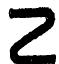
\includegraphics[keepaspectratio]{images/part001_40fd7be3.jpg}}

X 到 \(X'\) 上的等距映射当然是 X 的一致结构（相应地，拓扑）到 \(X'\) 的一致结构（相应地，拓扑）上的同构；这些命题的逆命题不成立，互不相同的等价度量的存在性（ \(\S\) 1，第 2 号）就表明了这一点。

设 X 是一个度量空间，d 是 X 上的度量。对每个 a \textgreater{} 0 ，用 \(V_{a}\) 表示 \(X \times X\) 的由所有点对 \((x, y)\) （满足 \(d(x, y) < a\) ）组成的子集，用 \(W_{a}\) 表示 \(X \times X\) 的由所有点对 \((x, y)\) （满足 \(d(x, y) \leqslant a\) ）组成的子集。当 a 取遍所有实数 \textgreater{} 0 组成的集（或仅仅取遍一个趋于 0 的 \textgreater{} 0 数列）时，诸集 \(V_{a}\) （相应地，\(W_{a}\) ）构成 X 的一致结构的开（相应地，闭）围域的一个基本系，这是由 d 的连续性得到的（§ 1，第 3 号）。我们有 \(\overline{V}_{a} \subset W_{a}\) ，但这两个集未必相同。

与 \(R^{n}\) 上欧氏距离的情形类比，集 \(\mathrm{V}_{a}(x)\) {[}相应地，\(\mathrm{W}_{a}(x)\) {]}称为以 x 为中心、以 a 为半径的开球（相应地，闭球）；它是 X 中的一个开（相应地，闭）集。又，由所有点 \(y \in X\) （满足 \(d(x, y) = a\) ）组成的集称为以 x 为中心、以 a 为半径的球面；它是一个闭集。由上所述，当 a 取遍所有实数 \textgreater0 组成的集或一个趋于 o 的 \textgreater0 数列时，以 x 为中心、以 a 为半径的开球（相应地，闭球）构成 x 的一个基本邻域系。

\pandocbounded{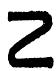
\includegraphics[keepaspectratio]{images/part001_d95d2d33.jpg}}

读者应当警惕，不要以为任意度量空间中的球与球面具有第六章，§ 2 中所研究的欧氏球与球面同样的性质。例如，开球的闭包未必是同一中心、同一半径的闭球；闭球的边界未必是同一中心、同一半径的球面；开球（或闭球）未必连通；而且球面可以是空集（参看习题 4）。

设 A 与 B 是度量空间 X 的任意两个非空子集。数

\[
d (\mathbf {A}, \mathbf {B}) = \inf _ {x \in \mathbf {A}, y \in \mathbf {B}} d (x, y)
\]

称为集合 A 与 B 之间的距离。特别地，我们用 \(d(x, \mathbf{A})\) 表示集合 \(\{x\}\) 与集合 A 之间的距离；它称为点 x 到集合 A 的距离。于是

\[
d (x, \mathrm{A}) = \inf _ {y \in \mathrm{A}} d (x, y)
\]

由此得

\[
d (\mathbf {A}, \mathbf {B}) = \inf _ {x \in \mathbf {A}} d (x, \mathbf {B})
\]

（第四章，§ 5，第 4 号，命题 9）。

注。若 \(d(x, \mathrm{A}) = a\) ，可能发生 A 中没有到 \(x\) 的距离等于 \(a\) 的点的情形。然而，若 A 是紧的，这种情形绝不会出现，因为这时魏尔斯特拉斯定理（第四章，§6，第 1 号，定理 1）表明，存在 \(y \in \mathrm{A}\) 使得 \(d(x, \mathrm{A}) = d(x, y)\) 。

命题 2. \(d(x, \mathbf{A}) = 0\) 与 \(x \in \overline{\mathbf{A}}\) 这两个陈述等价。

因为 \(d(x, \mathbf{A}) = 0\) 表明：球 \(\mathbf{V}_a(x)\) 与 \(\mathbf{A}\) 相交，无论 \(a > 0\) 取何值；而这等价于 \(x \in \overline{\mathbf{A}}\) 。

命题 3. 函数 \(d(x, \mathbf{A})\) 在 \(\mathbf{X}\) 上一致连续。

设 \(x\) 与 \(y\) 是 \(\mathbf{X}\) 中任意两点；则对任意给定的 \(\varepsilon > 0\) ，存在 \(z \in \mathbf{A}\) 使得 \(d(y, z) \leqslant d(y, \mathbf{A}) + \varepsilon\) ，因而

\[
d (x, z) \leqslant d (x, y) + d (y, z) \leqslant d (x, y) + d (y, A) + \varepsilon
\]

由三角不等式。

更有 \(d(x, \mathbf{A}) \leqslant d(x, y) + d(y, \mathbf{A}) + \varepsilon\) ，且由于 \(\varepsilon\) 是任意的，由此得 \(d(x, \mathbf{A}) \leqslant d(x, y) + d(y, \mathbf{A})\) 。类似地有

\[
d (y, \mathbf {A}) \leqslant d (x, y) + d (x, \mathbf {A}),
\]

从而

\[
\left| d (x, \mathbf {A}) - d (y, \mathbf {A}) \right| \leqslant d (x, y),\tag{2}
\]

由此即得结论。

注。可以有 \(d(\mathbf{A}, \mathbf{B}) = 0\) ，对某两个子集 \(\mathbf{A}, \mathbf{B}\) （\(\mathbf{X}\) 的子集）而言，它们满足 \(\overline{\mathbf{A}} \cap \overline{\mathbf{B}} = \emptyset\) ，只要这两个子集都不由单独一个点组成。例如，在实直线 \(\mathbf{R}\) 上，整数 \(> 0\) 组成的集与序列 \((n + 1/2n)_{n \geqslant 1}\) 的点组成的集是两个互不相交的闭集，它们之间的距离为零。

然而，若 A 紧且 B 闭，则关系 \(d(A, B) = 0\) 蕴含 \(A \cap B \neq \varnothing\) ，因为借助关系式

\[
d (\mathbf {A}, \mathbf {B}) = \inf _ {x \in \mathbf {A}} d (x, \mathbf {B})
\]

由命题 3 与魏尔斯特拉斯定理可知，存在 \(x_0 \in \mathbf{A}\) 使得 \(d(x_0, \mathbf{B}) = d(\mathbf{A}, \mathbf{B}) = 0\) ，从而（命题 2）\(x_0 \in \mathbf{B}\) 。

X 的非空子集 A 的直径是数（有限或等于 +∞）

\[
\delta (\mathbf {A}) = \sup _ {x \in \mathbf {A}, y \in \mathbf {A}} d (x, y).
\]

``W \(_{a}\) -小集''（第二章，§ 3，第 1 号）的概念与直径 \(\leqslant a\) 的集的概念相同。非空集 A 由单独一个点组成的必要充分条件是 \(\delta(\mathbf{A}) = 0\) 。

X 的子集 A （关于度量 d）称为有界的，如果它的直径有限；等价地，如果对每个点 \(x_{0} \in X\) ，A 都包含在以 \(x_{0}\) 为中心的一个球中。有界集的每个子集是有界的，且有限个有界集的并是有界集。

注意，X 的一个子集可以关于度量 d 有界，而关于与 d 等价的某个度量无界（参看 § 1，第 2 号）。

